\documentclass{article} % For LaTeX2e
\usepackage{nips13submit_e,times}
%\usepackage{hyperref}
\usepackage{url}
\usepackage{graphicx}
%\documentstyle[nips13submit_09,times,art10]{article} % For LaTeX 2.09
%\usepackage{authblk}

\title{10-601B Group Project Midway Report}

\author{
Liruoyang, Yu\\
MISM\\
\texttt{magicyuli@cmu.edu}
\and
Yilong, Chang\\
MISM\\
\texttt{yilongc@andrew.cmu.edu}
}


% The \author macro works with any number of authors. There are two commands
% used to separate the names and addresses of multiple authors: \And and \AND.
%
% Using \And between authors leaves it to \LaTeX{} to determine where to break
% the lines. Using \AND forces a linebreak at that point. So, if \LaTeX{}
% puts 3 of 4 authors names on the first line, and the last on the second
% line, try using \AND instead of \And before the third author name.

\newcommand{\fix}{\marginpar{FIX}}
\newcommand{\new}{\marginpar{NEW}}

%\nipsfinalcopy % Uncomment for camera-ready version

\begin{document}
\maketitle
\begin{abstract}
This report summarizes the halfway results of the 10-601B image classification group project. This report will introduce the classifiers we implemented, and then focus on the implementation methods and the experiment results.
\end{abstract}

\section{Introduction}
Up to this point, we trained and tested two classifiers, SVM and Neural Network. The dataset we used for training is a subset of 5000 images from CIFAR-10. We used VLFeat to extract HoG from images and then feed the extracted features to our classifiers.

We achieved 60\% and 50\% accuracy on Autolab test using SVM and Neutral Network respectively.

\subsection{Motivation}

There are three reasons why we chose SVM. First is that image data is usually not linearly separable in the original feature space, and kernel SVM can deal with this kind of dataset pretty well. Second, the training of SVM is a convex optimization problem, which made it efficient to train. Three, SVM has relatively higher resistance to over-fitting because of the maximization of the margin. And it's easy to adjust C to avoid over-fitting.

On the other hand, Neural Network is a non-paramateric model and therefore, is easy to use and understand.

\subsection{Background and Related Work}

"Image classification refers to the task of extracting information classes from a multiband raster image". And CIFAR-10 is an established dataset consisting of 60000 32$\times$32 color images in 10 classes used for the purpose of studying Image classification. 

\subsubsection{Related Work}

Kernel SVM has proven to be effective in the image classification field\cite{chapelle1999support} and was the go-to method before Convolutional Neural Network (CNN) exhibited its great power.

In recent years, Convolutional Neutral Network achieved great performance in image classification. Some recent implementations of Convolutional Neural Network have achieved state-of-the-art performance on the CIFAR-10 images, which are our target dataset. These works include a most recent model in Torch\cite{torch}, a 92.45\% accuracy. The Deeply Supervised Networks\cite{lee2014deeply}, by introducing a "companion" objective functions at each individual hidden layer they achieved an accuracy of 91.78\%. The Network in Network\cite{minlin2014network}, in which the authors built micro neural networks to abstract the data within the receptive field and obtained a 91.2\% accuracy.


\section{Method}

\subsection{Feature Engineering}

We used VLFeat to extract the Histogram of Oriented Gradient (HoG) of images, and use them as the features. HoG summarizes the magnitude of gradients along different directions at different positions of a image, which can reflect color and brightness changes.

\subsection{Data Preprocessing}
In order to prevent over-fitting and improve the training efficiency, we applied PCA to the extracted HoG data. Before PCA, there were 2304 feature dimensions. After PCA, we preserved the first 700 components for the Neural Network, which can explain 98\% of the variance; and 900 for SVM, which can explain more than 99\%.

\subsection{SVM}

\subsubsection{Training}

Since there 10 classes of images, we adopted the 1 vs all strategy, i.e. training 10 classifiers based on the 10 labels we have.

We trained each classifier by maximizing the following dual problem of the objective function of SVM
\begin{equation}
W(\alpha)=\sum_{i=1}^{N}\alpha_{i}-\frac{1}{2}\sum_{i,j=1}^{N}\alpha_{i}\alpha_{j}y_{i}y_{j}K(\mathbf{x_{i}},\mathbf{x_{j}})
\end{equation}
\begin{equation}
0<\alpha_{i}<C
\end{equation}
,where $\mathbf{x_{i}}$ is the feature vector of a training sample after HoG and PCA, $y_{i}=1$ or $-1$ indicating whether $\mathbf{x_{i}}$ belongs to that class, $K(\mathbf{x_{i}},\mathbf{x_{j}})$ is the kernel trick. And we used the Gaussian Kernel as the kernel function
\begin{equation}
K(\mathbf{x_{1}},\mathbf{x_{2}})=e^{-\frac{||\mathbf{x_{1}}-\mathbf{x_{2}}||^{2}_{2}}{2\sigma^{2}}}
\end{equation}

We used quadprog() in Matlab to find the $\mathbf{\alpha}$ that maximizes function (1), then compute the bias as
\begin{equation}
b=\frac{\sum_{i=1}^{N}\alpha_{i}y_{i}}{\#~of~\alpha_{i}\neq{0}}
\end{equation}

\subsubsection{Predicting}

We predicted the class $c$ for new samples based on
\begin{equation}
c=\arg\max_{c}\sum_{i=1}^{N}\alpha_{i,c}y_{i,c}K(\mathbf{x_{i}},\mathbf{x_{new}})+b_{c}
\end{equation}

\subsubsection{Future Plan}
Next, we plan to experiment with different kernel functions, e.g. $\chi^{2}$ RBF, Laplacian RBF, because the HoG features we're using are discrete. C should be further tuned, too, because we observed that it's somewhat over-fitted the training set, i.e. it achieved 100\% accuracy on the training set, while only 60\% on the Autolab test set.

Yet another more sophisticated thing to try is to combine Neural Network with SVM, i.e. to substitute the output layer with SVM. The intuition behind this is that Neural Network can work as a more complex feature selector extracting latent features from the images, and then feed the them into SVM.


\subsection{Neural Network}
We implemented the basic Neural Network. That is one input layer, one hidden layer and one output layer. Since we used 700 features, the number of input nodes was 700. After testing different number of hidden nodes, we chose a number around 50. And the number of output nodes was ten. We  used incremental mode gradient descent to train the data for prediction.${We used our model to train two different pairs of weights for submission.}$

\subsubsection{Training}
During the training process, we calculated the error for each training example at output layer as: 
\begin{equation}
\varepsilon_{k} = t_{k} - o_{k}
\end{equation}
where $o_{k}$ is the observed unit output, $t_{k}$ is the target output.

To minimize error, we used RMSE as our performance function:
\begin{equation}
RMSE = \sqrt{\frac{1}{n}\sum_{k=1}^{n}\varepsilon_{k}^2}
\end{equation}
And we would stop iteration once the change rate of RMSE dropped to a threshold.

\subsubsection{Predicting}
We predicted the class of test data with:
\begin{equation}
y=\arg\max_{c}o_{c}
\end{equation}
where $o_{c}$ is the output for class c.

\subsubsection{Future Plan}
In the next phase, we will implement Batch mode Gradient Descent and compare the performance of Batch mode and Incremental mode. As to over-fitting problem, we will implement some other regularization methods to see if better performance will be achieved.

After that we will try to build a more advanced Neural Network model. Maybe we will challenge ourselves with Convolutional Neural Network.

\subsection{Evaluation}

We evaluated our classifier by accuracy on the validation set and the test set on Autolab. And when training Neutral Network, we evaluated the model we trained by the RMSE on the training set.

We also leveraged validation to select the optimal hyperparameters as described in section \ref{experiments}, Experiments and Results.

\section{Experiments and results}
\label{experiments}

\subsection{SVM}

\subsubsection{Linear SVM vs Kernel SVM}
We experimented with both Linear SVM and Kernel SVM, and it turned out that Linear SVM achieved best accuracy of 53\% on the validation set, whereas Kernel SVM achieved 61.8\%.

\subsubsection{Hyperparameter Selection}

There are two hyperparameters for Gaussian Kernel SVM, namely $C$ and $\sigma$. We selected these hyperparameters by validation. We separated the 5,000 samples in the training set into one training set of 4,000 samples and one validation set of 1,000 samples.

We selected $\sigma$ and $C$ based on the accuracy on the validation set, as shown in Figure \ref{figure1} for $\sigma$ and Figure \ref{figure2} for $C$. 

The final $\sigma$ and $C$ we selected were 1.9 and 100, which achieved 61.8\% accuracy on the validation set.

\subsubsection{Autolab submission}
Our Kernel SVM classifier achieved 60\% accuracy on Autolab test set.

\begin{figure}[ht!]
	\centering
	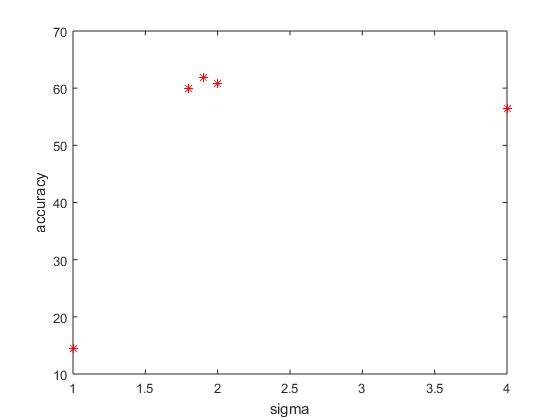
\includegraphics[width=90mm]{sigma.jpg}
	\caption{Validation set accuracy under different sigma\label{figure1}}
\end{figure}

\begin{figure}[ht!]
	\centering
	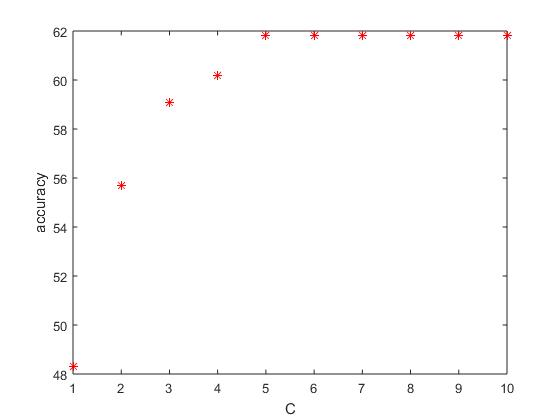
\includegraphics[width=90mm]{C.jpg}
	\caption{Validation set accuracy under different C\label{figure2}}
\end{figure}

\subsection{Neural Network}
We trained two models using different loss functions. In both training processes we first initialized the weights vectors $\mathbf{w}$, which was the weight vector between input layer and hidden layer, and $\mathbf{u}$, the weight vector between hidden layer and output layer with random number $\sim$ $N$(0, $D$), where $D$ is the size of training set. 
\subsubsection{Basic Neural Network}
In the first model, we set a fixed learning rate at:
\begin{equation}
\eta = 2
\end{equation}
We used the 4000 samples to train. Once the change rate of RMSE was less than 0.0005, we would stop the iteration. 

\subsubsection{Regularized Neural Network}
In the second model, we added two bias vectors $\mathbf{b1}$ and  $\mathbf{b2}$ with initial values from [-0.5, 0.5], and updated these two vectors together with weight vectors. 

This time, we set the learning rate at:
\begin{equation}
\eta = \frac{2}{\sqrt{m}},
\end{equation}
where m is the current number of epoch. 

To avoid over-fitting, we regularized using Simple Weight Decay:
\begin{equation}
\mathbf{w}\rightarrow\mathbf{w_0}-\frac{\eta\lambda}{n}
\end{equation}
where $\mathbf{w_0}$ is the weight vector before regularization.

After some trials, we set the parameters and trained the model with all the 5000 samples.

\subsubsection{Results: Basic Neural Network}
The highest accuracy on local machine was 54.1\%. We submitted a model of 52.8\% on Autolab and the result was 48.4\%.
\subsubsection{Results: Regularized Neural Network}
The accuracy on training data before regularization was around 90\%, but decreased to around 78\% after regularization. And the test result on Autolab was 50\%.



\section{Conclusion}
Although we just implemented relatively simple models of Kernel SVM and Neural Network, they perform pretty well on this task. We think this is because they're both non-linear classifiers. However, this tends to lead to over-fitting, as we observed in Neural Network, and a little bit in SVM. After tuning they should perform better.

We still plan to try Logistic Regression or Bayesian Network.



\bibliographystyle{abbrv}
\bibliography{nips2013}  % sigproc.bib is the name of the Bibliography
\end{document}
